\section{Experiment 2: Simulated Data with Latent Structure}

In the second simulation experiment, we focused on data generated from a Factor Analysis model.
The data social scientists analyse are often a collection of items measuring different latent constructs, 
a characteristic that is likely to impact imputation performances.
In Experiment 2, we investigated the performances of the missing data treatments in relation to three experimental factors.
First, the dimensionality of the data was controlled by the number of latent variables $l$ (10, 100).
5 items were generated as measurements of each latent variable, resulting in either 50 or 500 items.
Second, factor loadings were defined as a 2-level random experimental factor (high, low).
High factor loadings were drawn from a uniform distribution between (0.9, 0.97), while low factor loadings
were drawn from a uniform distribution between (0.5, 0.6).
Third, the proportion of missing values was defined as a fixed experimental factor with two levels: 0.1 or 0.3.
Table \ref{tab:condExp2} summarizes the eight resulting conditions.

Data with sample size $n=200$ were independently generated 1,000 times for each condition.
For each replicate, missing values were imposed and then each missing data treatment was used to obtain estimates 
for the parameters of a complete-data analysis model.
With a sample size fixed at 200, conditions with $l = 10$ resulted in a low-dimensional settings, while conditions 
with $l = 100$ resulted in a high-dimensional settings.

\begin{table}
\tbl{Summary of conditions for Experiment 2.}
	{
	\begin{tabular}{l c c c c c c } 
		\toprule
		condition & label & n & p & l & pm & $\lambda$ range \\
		\midrule
		1 & low-dim-low-pm-high-$\lambda$ & 200 & 50 &  10 &  0.1 & [0.9, 0.97] \\
		2 & high-dim-low-pm-high-$\lambda$ & 200 & 500 & 100 & 0.1 & [0.9, 0.97] \\
		3 & low-dim-high-pm-high-$\lambda$ & 200 & 50 &  10 &  0.3 & [0.9, 0.97] \\
		4 & high-dim-high-pm-high-$\lambda$ & 200 & 500 & 100 & 0.3 & [0.9, 0.97] \\
		5 & low-dim-low-pm-low-$\lambda$ & 200 & 50 &  10 &  0.1 & [0.5, 0.6]  \\
		6 & high-dim-low-pm-low-$\lambda$ & 200 & 500 & 100 & 0.1 & [0.5, 0.6]  \\
		7 & low-dim-high-pm-low-$\lambda$ & 200 & 50 &  10 &  0.3 & [0.5, 0.6]  \\
		8 & high-dim-high-pm-low-$\lambda$ & 200 & 500 & 100 & 0.3 & [0.5, 0.6]  \\
		\bottomrule
	\end{tabular}
	}
\label{tab:condExp2}
\end{table}

\FloatBarrier % stops table:condSum leaving its own section

\subsection{Simulation Study Procedure}

%\paragraph{Data Generation}
	For each replication, an observed data matrix $\bm{Z}_{n \times p}$ was created based on a Confirmatory 
	Factor Analysis model.
	Each of $l$ latent variables was assumed to be measured by 5 items, for a total of $p = 5*l$ 
	columns in $\bm{Z}$.
	Values on the items for the $i$-th observation were obtained with the following measurement 
	model:
%
	\begin{equation}
		\bm{z}_i = \bm{\Lambda} \bm{\xi}_{i.} + \bm{\delta}_{i.}
	\end{equation}
%
	where $\bm{z}_i$ is a vector of $5*l$ items scores for observations $i = 1, ..., n$;
	$\bm{\Lambda}$ is the $(5*l) \times l$ matrix of factor loadings; $\bm{\xi}_{i.}$ is a vector of $l$ latent scores 
	for observation $i$; and $\bm{\delta}_{i.}$ is a vector of $5*l$ uncorrelated measurement errors sampled from a 
	multivariate normal distribution centered around a mean vector of 0s and with a diagonal covariance matrix $\bm{\Theta}$.
	All items were centered around a mean of 5.
	For notation and model specification the interested reader may refer to \cite{bollen:1989}.

	The latent scores in $\bm{\xi}_{i.}$ were sampled from a multivariate normal distribution centered around 
	0, and with a covariance matrix $\bm{\Psi}$, with diagonal elements equal to 1 and off-diagonal elements 
	equal to correlation between latent factors. 
	In particular, the first 4 latent variables were highly correlated ($\rho = .6$), the second block of 4 
	latent variables were weakly correlated ($\rho = .3$), while the remaining $l-8$ latent variables were 
	uncorrelated.

	The matrix $\bm{\Lambda}$ defined a simple latent structure where each item loaded on only 1 factor (5 items 
	for each latent variable).
	Both the item and latent factor variances were set to 1 so that the measurement error variance was defined as 
	$var(\delta) = 1 - \lambda^{2}$.
	This specification allowed factor loadings $\lambda_{ij}$, with $i = 1, ..., n$ and $j = 1, ..., l$, to be
	defined as standardized values between 0 and 1.
	The exact values for the latent factors were drawn for each repetition from a uniform distribution 
	with bounds defined by the condition.

%\paragraph{Missing Data Imposition}

	Item non-response was imposed on 10 items in $\bm{Z}$ using Equation \ref{eqn:rm} to define the probability
	of a value being missing.
	The items targeted by the missing data imposition measured the first two highly correlated latent variables
	($l = 1, 2$).
	The predictors included in $\tilde{Z}$ were the latent scores for the other two highly correlated latent 
	variables ($l = 3, 4$).
	
%\paragraph{Imputation}
	
	Missing values were treated according to all the methods previously described.
	The imputation methods were parametrized as in Experiments 1.
	50 iterations were sufficient for convergence of all MI methods except blasso, which required approximately 
	2,000 iterations for convergence.

%\paragraph{Analysis}
	
	The substantive model of interest in Experiment 2 was a saturated model that estimated means,
	variances, and covariances of the raw items with missing values.
	Furthermore, the true Factor Analysis model for the same items was estimated to see how the 
	factor loadings were recovered after imputation.

\subsection{Results}
	To assess the performances of the methods, we used the same comparison criteria described for Experiment 1.
	Figures \ref{fig:exp2bias14} and \ref{fig:exp2cir14} report the maximum, average, and minimum $|\text{PRB}|$ and 
	CIC obtained with each missing data treatment method for each parameter type (mean, variance, and covariance) in 
	the conditions with high factor loadings.
	Figures \ref{fig:exp2bias58} and \ref{fig:exp2cir58} report the same results for the conditions with low 
	factor loadings.
	In the supplementary material you may find the figures reporting the raw PRBs and CICs for every parameter.

	\paragraph{Means}
	All the imputation methods resulted in unbiased estimation of the item means with maximum $|\text{PRB}| < 10\%$ 
	in all conditions.
	In particular, IURR, MI-PCA, and MI-OP exhibited the smallest bias, and only CC analysis led to substantial 
	bias of the means.
	When factor loadings were large, DURR, IURR and MI-PCA resulted in little to no deviations from nominal 
	coverage, while blasso, bridge, MI-CART, MI-RF, and missForest led to significant under-coverage of the 
	true means when the proportion of missing cases was high (columns 3 and 4 in the figures).
	In the conditions with lower factor loadings, all methods performed worse, but relative performances remain
	unchanged.
	IURR, MI-PCA, and MI-OP exhibited again the smallest bias and deviation from nominal coverage rates.
	However, MI-PCA and MI-OP were the only methods returning small deviations from nominal coverage rates in the 
	high-dim-high-pm-low-$\lambda$ condition.
	
	\paragraph{Variances}
	All MI methods, except bridge, resulted in acceptable estimation bias for the item variances in all conditions
	with large factor loadings.
	The least biased estimates were obtained by IURR, MI-PCA, and MI-OP.
	As for CIC, for high-pm conditions (columns 3 and 4), only IURR and MI-PCA maintained CICs mostly within the 
	range (0.94, 0.96), while blasso and the MI tree-based methods led to mild to extreme under-coverage 
	(maximum CIC < 90\%).
	Single data approaches, missForest and CC, showed again extreme bias and large significant CI under-coverage 
	in almost all conditions.
	The large bias and low coverage for the item variances that afflicted MI-PCA in the multivariate-normal set up 
	(figures \ref{fig:exp1bias} and \ref{fig:exp1cir}) was not present in figures \ref{fig:exp2bias14} and 
	\ref{fig:exp2cir14}.
	However, that pattern reappeared in the conditions with low factor loadings (see figures \ref{fig:exp2bias58} 
	and \ref{fig:exp2cir58}).

	\paragraph{Covariances}
	For all the conditions with high factor loadings, IURR and DURR showed acceptable covariance biases 
	(largest $|\text{PRB}|<10\%$).
	However, they led to large covariance bias in all the conditions with low factor loadings 
	(see Figures \ref{fig:exp2bias58}).
	As in Experiment 1, MI-PCA resulted in the lowest bias and deviation from nominal coverage of the true 
	item covariances.
	The largest $|\text{PRB}|$ with MI-PCA was smaller than the $10\%$ threshold in all conditions, and the 
	average CIC fell within the interval (0.94, 0.96) in almost all conditions.
	All other methods led to large bias and mild-to-extreme significant covariance under-coverage 
	in all conditions.

\begin{figure}
	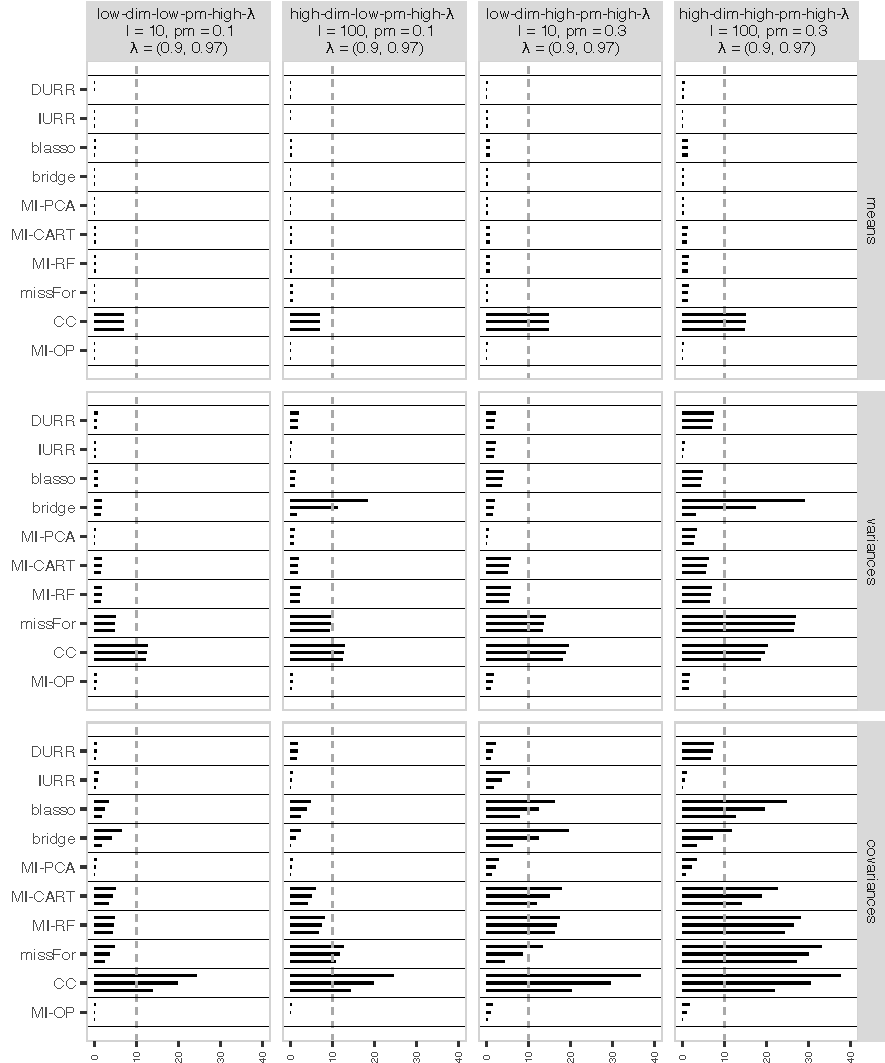
\includegraphics{\pathFIG/exp2_semR_bias_14_summy.pdf}
\caption{
	Maximum, average, and minimum absolute Percent Relative Bias ($|\text{PRB}|$) for item means, variances, 
	and covariances in the conditions of Experiment 2 with high factor loadings.
	For each method, the maximum, average, and minimum PRB are reported in this order.	
}
\label{fig:exp2bias14}
\end{figure}

\begin{figure}
	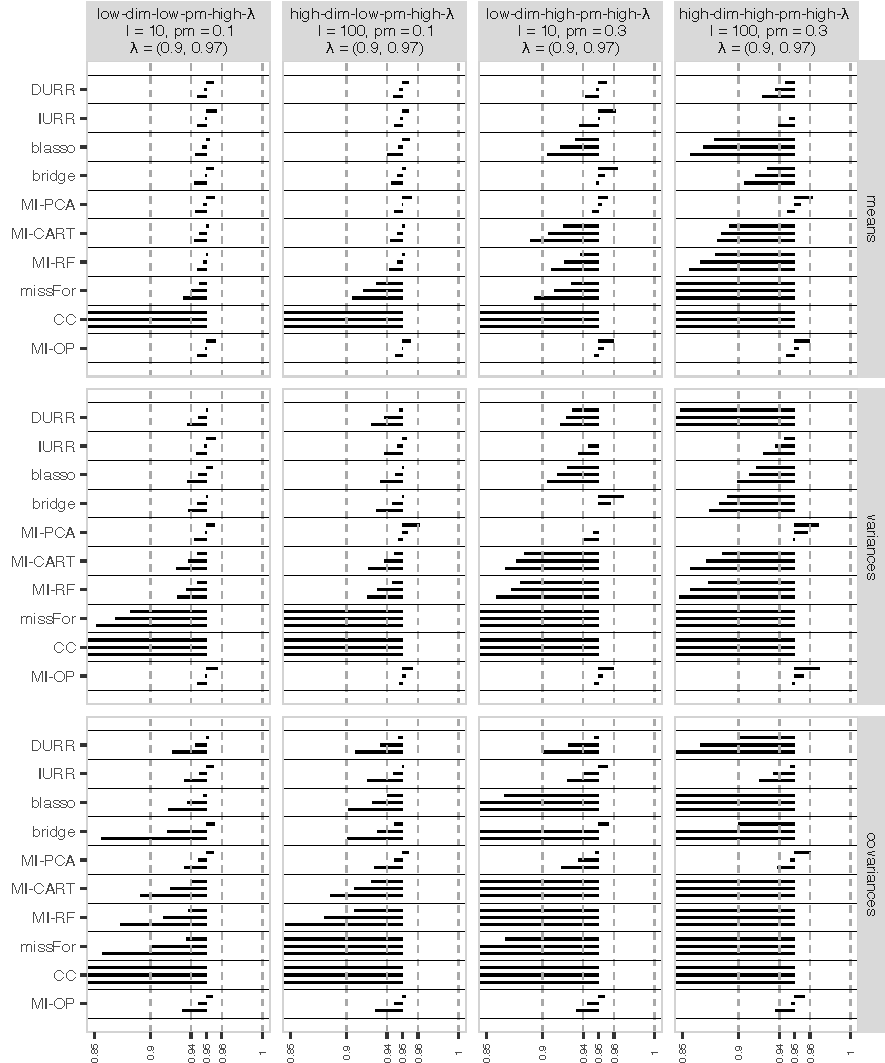
\includegraphics{\pathFIG/exp2_semR_ci_14_summy.pdf}
\caption{
	Maximum, average, and minimum CIC for item means, variances, and covariances in Experiment 2
	in the conditions of Experiment 2 with high factor loadings.
	For each method, the maximum, average, and minimum are reported in this order.
}
\label{fig:exp2cir14}
\end{figure}

\begin{figure}
	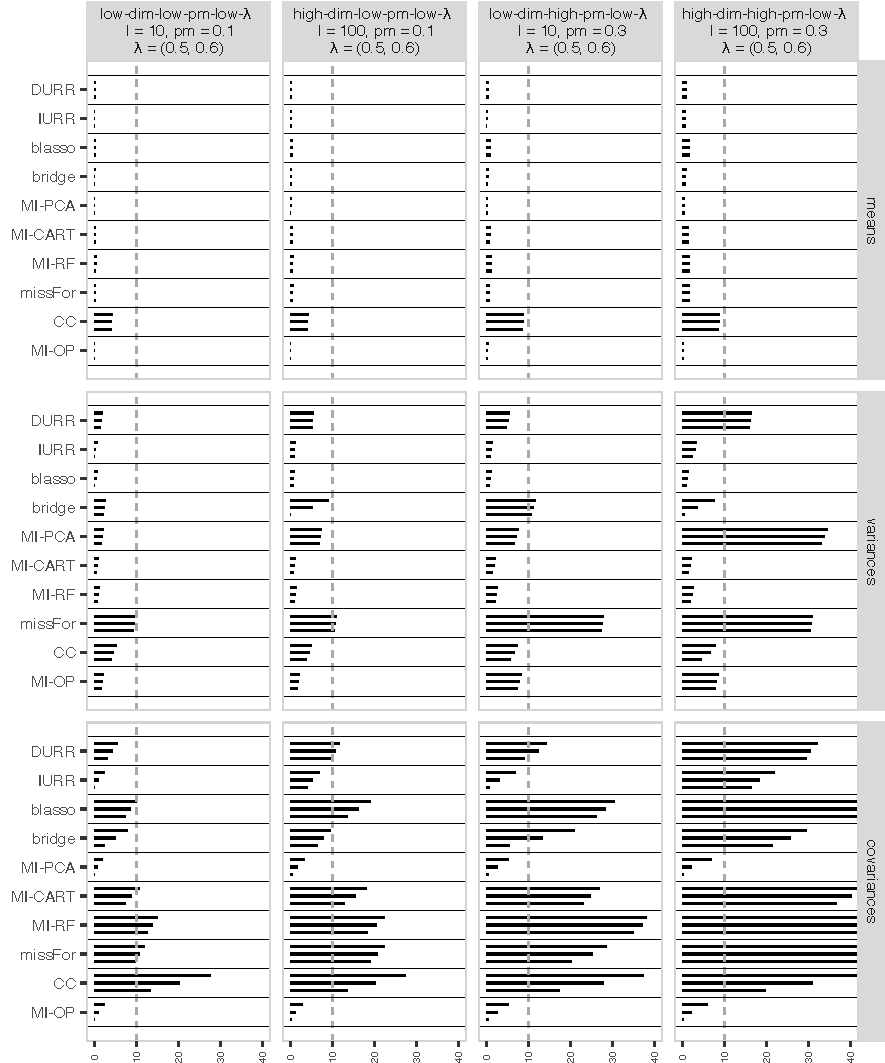
\includegraphics{\pathFIG/exp2_semR_bias_58_summy.pdf}
\caption{
	Maximum, average, and minimum absolute Percent Relative Bias ($|\text{PRB}|$) for item means, variances, 
	and covariances in the conditions of Experiment 2 with low factor loadings.
	For each method, the maximum, average, and minimum are reported in this order.	
}
\label{fig:exp2bias58}
\end{figure}

\begin{figure}
	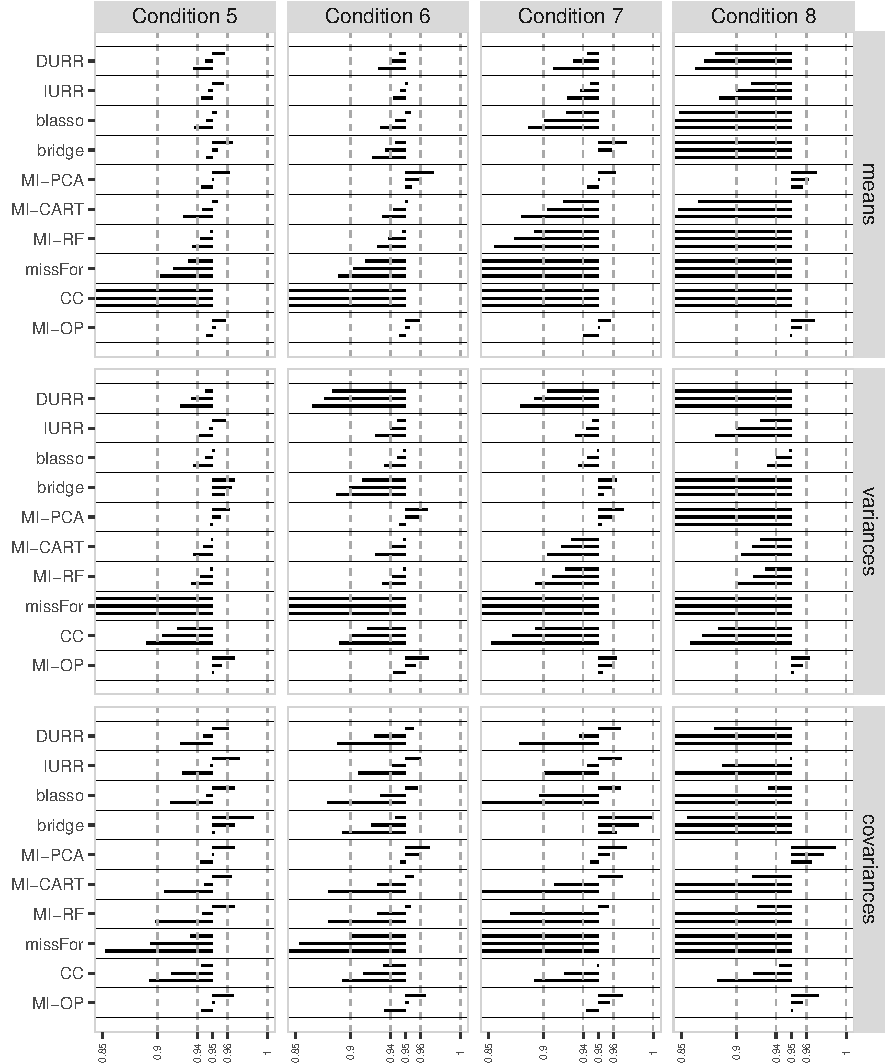
\includegraphics{\pathFIG/exp2_semR_ci_58_summy.pdf}
\caption{
	Maximum, average, and minimum CIC for item means, variances, and covariances in the conditions of 
	Experiment 2 with low factor loadings.
	For each method, the maximum, average, and minimum are reported in this order.
}
\label{fig:exp2cir58}
\end{figure}

\FloatBarrier

	\paragraph{Factor Loadings}
	Figure \ref{fig:exp2fl14} reports the maximum, average, and minimum absolute PRB values for all the factor 
	loadings estimated by the Confirmatory Factor Analysis described above.
	IURR, MI-PCA, and MI-OP, outperformed all other methods by producing virtually unbiased estimates of the 
	factor loadings in all conditions.
	However, MI-PCA outperformed IURR when factor loadings were low (panel b), maintaining inconsequential 
	biases even when data were high-dimensional and the proportion of missing values was high
	(high-dim-high-pm-low-$\lambda$).
	Blasso and MI-RF were the MI methods leading to the largest biases for this parameter type.
	Both of them resulted in extreme bias in the high-pm-low-$\lambda$ conditions with minimum $|\text{PRB}| > 10\%$.

\begin{figure}
	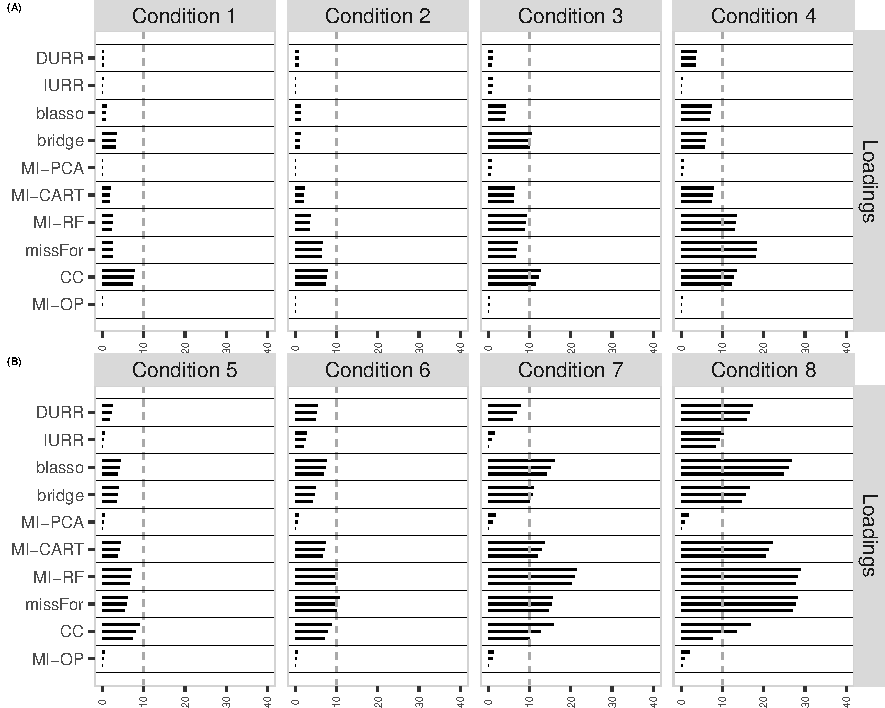
\includegraphics{\pathFIG/exp2_CFA_lambda_BPR_summy.pdf}
	\caption{
		Maximum, average, and minimum absolute Percent Relative Bias ($|\text{PRB}|$) for factor loadings
		in Experiment 2.
		For each method, the maximum, average, and minimum are reported in this order.	
		}
\label{fig:exp2fl14}
\end{figure}

\FloatBarrier % stops fig:exp2fl to leave its section

